\subsection{Dataset}
We utilized the MinneApple dataset, collected at the University of Minnesota's Horticultural Research Center (HRC). The dataset contains 1,000 images, which contain approximately 41,000 tagged instances. With a Samsung Galaxy S4 phone, \cite{Haeni2020} took videos of the apple trees moving smoothly on the sunny side, and intercepted every fifth frame of as training datasets and every thirtieth frame as test datasets.

In contrast to COCO, ImageNet, and PASCAL VOC, MinneApple focuses on detecting small objects in cluttered environments, with objects occupying 0.17\% of the image size. The average object categories and numbers of objects in each image for these datasets are summarised in Tab.~\ref{tab:categories}. MinneApple has more instances in a category (41.2), whilst it has fewer categories (1.5). In addition, the MinneApple dataset contains only full resolution images, and the developers took into account the variety of apples and lighting conditions so as to avoid misfitting. 

\begin{table}[htb]
\centering
\caption{Number of categories contained in each image and the number of instances of each category of the four datasets~\citep{Haeni2020}}
\label{tab:categories}
\resizebox{\textwidth}{!}{%
\begin{tabular}{@{}p{4.5cm}<{\centering} p{2.5cm}<{\centering} p{2.5cm}<{\centering} p{2.5cm}<{\centering} p{3cm}<{\centering}@{}}
\toprule
                       & MinneApple & COCO & ImageNet & PASCAL VOC \\ \midrule
Number of categories   & 1.5        & 3.5  & $\le 2$  & $\le 2$    \\
Instances per category & 41.2       & 7.7  & $\le 3$  & $\le 3$    \\ \bottomrule
\end{tabular}%
}
\end{table}


\subsection{Data Quality}
We employ the counting and the detection dataset from the MinneApple, which contains apples of different colours (red, green and yellow), as well as scenes with different light ratios. Most of the images in the counting dataset are $1\ Kb$ in size and have a resolution of no more than $100\times 100$ (Fig.~\ref{fig:counting dataset images}).

\begin{figure}[htb]
    \centering
    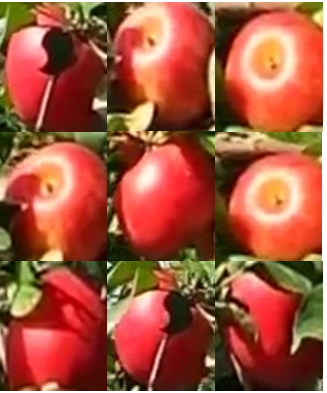
\includegraphics[width=0.3\textwidth]{images/counting_dataset.png}
    \caption{Images from the counting dataset~\citep{Haeni2020}}
    \label{fig:counting dataset images}
\end{figure}

As shown in Fig.~\ref{fig:masked_detection_image}, the annotations in the detection dataset are in the form of Mask. The resolution of the images in the detection dataset is $720\times 1280$, but a small proportion of the photos are overexposed, causing unclear colours and contours and improving the difficulty of the target detection task.

\begin{figure}[htb]
    \centering
    \subfigure[A image from the detection dataset]{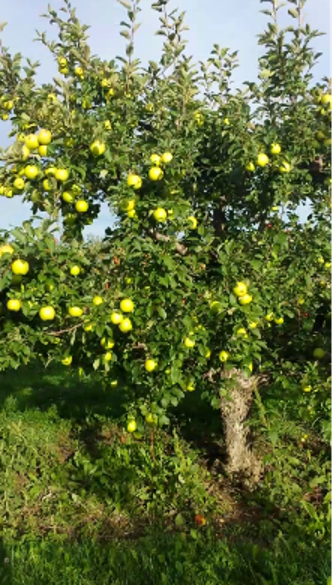
\includegraphics[width=0.3\textwidth]{images/mask_before.png}}
    \subfigure[The annotated image]{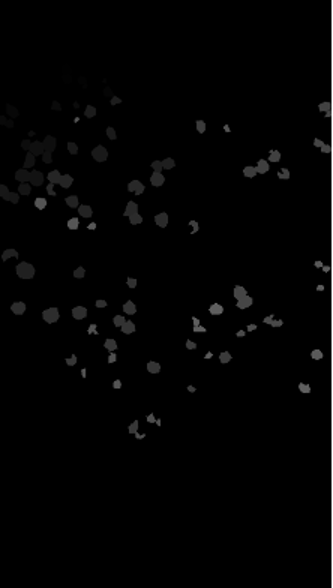
\includegraphics[width=0.3\textwidth]{images/mask_after.png}}
    \caption{A image from the detection dataset and the annotation——(a) a image from the detection dataset and (b) the annotated image}
    \label{fig:masked_detection_image}
\end{figure}



